\documentclass[twoside]{article}
\usepackage[utf8]{inputenc}
\usepackage[a4paper, total={6in, 8in}]{geometry}
\usepackage{fancyhdr}
\usepackage[english]{babel}
\usepackage{longtable}
\usepackage{graphicx}
\usepackage{parskip}
\usepackage{multicol}

\renewcommand{\familydefault}{\sfdefault}

\pagestyle{fancy}
\fancyhf{}
\rhead{Hannes Torstensson, Physics 1, NA21}
\lhead{Rolling Cylinders Down Slopes}
\fancyfoot[RO, LE] {\thepage}

\title{Rolling Cylinders Down Slopes - It Only Goes Downhill From Here}
\author{Hannes Torstensson \\ Physics 1, NA21}
\date{\today \\ Experiment performed 20th of September 2022}

\begin{document}

\maketitle

\section*{Purpose of the lab}
Investigating whether or not the formula $\Delta t = \frac{ 2 \times \Delta s }{ \sqrt{\frac{4 g \Delta h}{3}} } $ predicts time taken for a cylinder to roll down a slope with the non-circular face touching the slope.

\section*{Background}
We know that energy is always conserved, meaning that $E_{before} = E_{after}$, though the energy may not be in the same form. This can be used to derive the above formula. $\Delta E_{p}$ is change in potential energy, $\Delta E_{k}$ is change in kinetic energy, $\Delta E_{rot}$ is change in rotational energy, $m$ is mass, $g$ is 9.82, $\Delta h$ is the height, $v$ is velocity, $t$ is time, and $\Delta s$ is change in position.

\begin{multicols}{2}
\begin{center}
Finding the final velocity:

\end{center}
\[ \Delta E_{p} = \Delta E_{k} + \Delta E_{rot} \]
\[ mg \Delta h = \frac{mv^2}{2} + \frac{mv^2}{4} \]
\[ g \Delta h  = \frac{3v^2}{4} \]
\[ v = \sqrt{\frac{4g \Delta h}{3}} \] \break \break \break
\begin{center}
Finding the time taken:
\end{center}
\[ \Delta s = \frac{v+v_{0}}{2} \times \Delta t \]
\begin{center}
Since the cylinder is starting from a standstill, $v_{0}$ is equal to zero.
\end{center}
\[ \Delta s = \frac{v}{2 \Delta t} \]
\[ \Delta t = \frac{\Delta s}{\frac{1}{2}v} \]
\[ \Delta t = \frac{ 2 \times \Delta s }{ \sqrt{\frac{4 g \Delta h}{3}} } \]
\end{multicols}

\section*{Theoretical Prediction}
\begin{center}
	\begin{tabular}{ |p{3cm}|p{3cm}|p{3cm}| }
		\hline
			\multicolumn{3}{|c|}{Theoretical Prediction} \\
		\hline
			$\Delta s$ (m) & $\Delta h$ (m) & Theoretical Time (s) \\
		\hline
			0.50 & 0.02 & 1.95416 \\ \hline
			0.375 & 0.015 & 1.69235 \\ \hline
			0.25 & 0.01 & 1.38180 \\ \hline
			0.125 & 0.005 & 0.97708 \\ \hline
	\end{tabular}
\end{center}

\section*{Materials \& Method}
Materials used were: Metal sheet, cardboard box, metal cylinder, phone (timer), and ruler. Method: Begin by creating a slope using the metal sheet and cardboard box. Then measure the length of the metal sheet and the height of the cardboard box and record. Then roll the cylinder down the slope 10 times at 100\% of available slope, recording the time taken each time using a timer. Repeat for 75\%, 50\%, and 25\%.

\section*{Results}

\begin{center}
	\begin{tabular}{ |p{3cm}|p{3cm}|p{3cm}|p{3cm}|  }
		\hline
  	  \multicolumn{4}{|c|}{Results} \\
  	\hline
			$\Delta s$ (m) & $\Delta h$ (m) & Theoretical time (s) & Mean Experimental Time (s) \\
 	  \hline
 	    0.50 & 0.02 & 1.95416 & 1.6 \\ \hline
  	  0.375 & 0.015 & 1.69235 & 1.4 \\ \hline
  	  0.25 & 0.01 & 1.38180 & 1.3 \\ \hline
      0.125 & 0.005 & 0.97708 & 0.9 \\ \hline
	\end{tabular}
	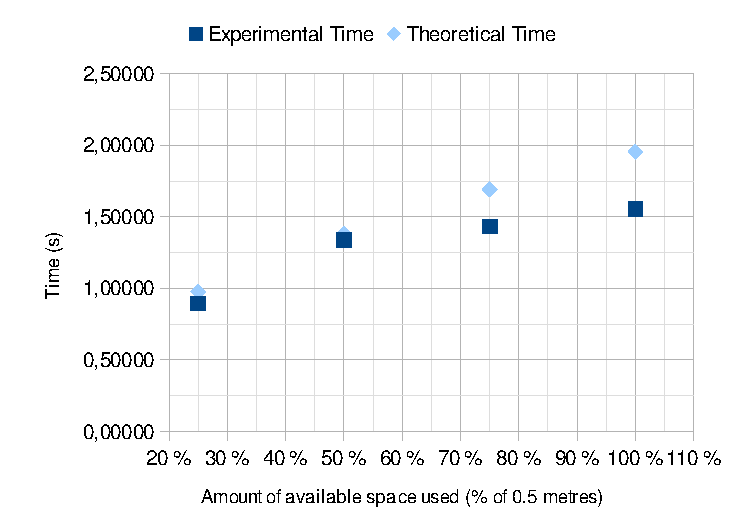
\includegraphics[width=10cm]{chart.pdf}
\end{center}

\section*{Discussion}
Our theoretical time predictions do not agree well with the experimental times we observed, and thus the experiment is inconclusive.

The accuracy can be quantified with the following formula, where $a$ is accuracy:
\[ a = \frac{\Sigma_{TheoreticalTimes}}{\Sigma_{Experimental Times}} \]
When we plug our numbers into that, we get the following calculation:
\[ a = \frac{1.95416+1.69235+1.38180+0.97708}{1.6+1.4+1.3+0.9} \]

Which works out to $a = 1.2$ after rounding to two significant figures. That means our prediction was wrong by an average of +20\%, which in other words means that our calculated theoretical times were, on average, 20\% longer than our measured experimental times.

This is rather surprising, as we would expect the experimental times to be longer than our theoretical times, since our theoretical prediction assumed a perfect cylinder with no friction. A possible source for this error is incorrect measurment of the time taken in our experiments, as humans do not have perfect reaction times.

One improvement of the experimental method would be to use an optical timer, a timer that starts and stops when, for example, laser beams are broken. A way of getting a more precise result would also be to have a better way of measuring distance, as school rulers are not known for extreme precision, especially not in the hands of highschoolers who would rather be at home sleeping.

Another way of mitigating the above outlined flaw would be to have a longer track for the cylinder to roll down, as that would make the error from the human factor less significant in the result, as the error would probably remain the same as the time taken increases.

Our theoretical prediction could be improved by accounting for friction in our equation, and by having more precise measuring tools for the distances, as outlined above.

\end{document}

